\chapter{SPRINT THREE - Exam and apply to become an instructor}
\minitoc
\newpage
\section*{Introduction}
\addcontentsline{toc}{section}{Introduction}
In this sprint, we will take a look at how the instructor can create an exam and how a user can apply to become an instructor.
\section{Sprint backlog}
%%%%%table
\begin{table}[H]
\centering
\caption{Product backlog}
\begin{tabular}{|p{1cm}|p{3cm}|p{6cm}|p{2cm}|}
\hline
\rowcolor{brown!18}\textbf{\large{ID}} & \textbf{\large{As a}} & \textbf{\large{I want to be able to}} & \textbf{\large{Priority}} \\
\hline
8& Instructor & Create an exam & High\\\hline
9& User & Apply to become an instuctor  & Normal \\\hline
\end{tabular}
\end{table}
%%%%%table
\section{Requirement analysis}
\subsection{Use case diagram}

\begin{figure}[!ht]
    \centering
    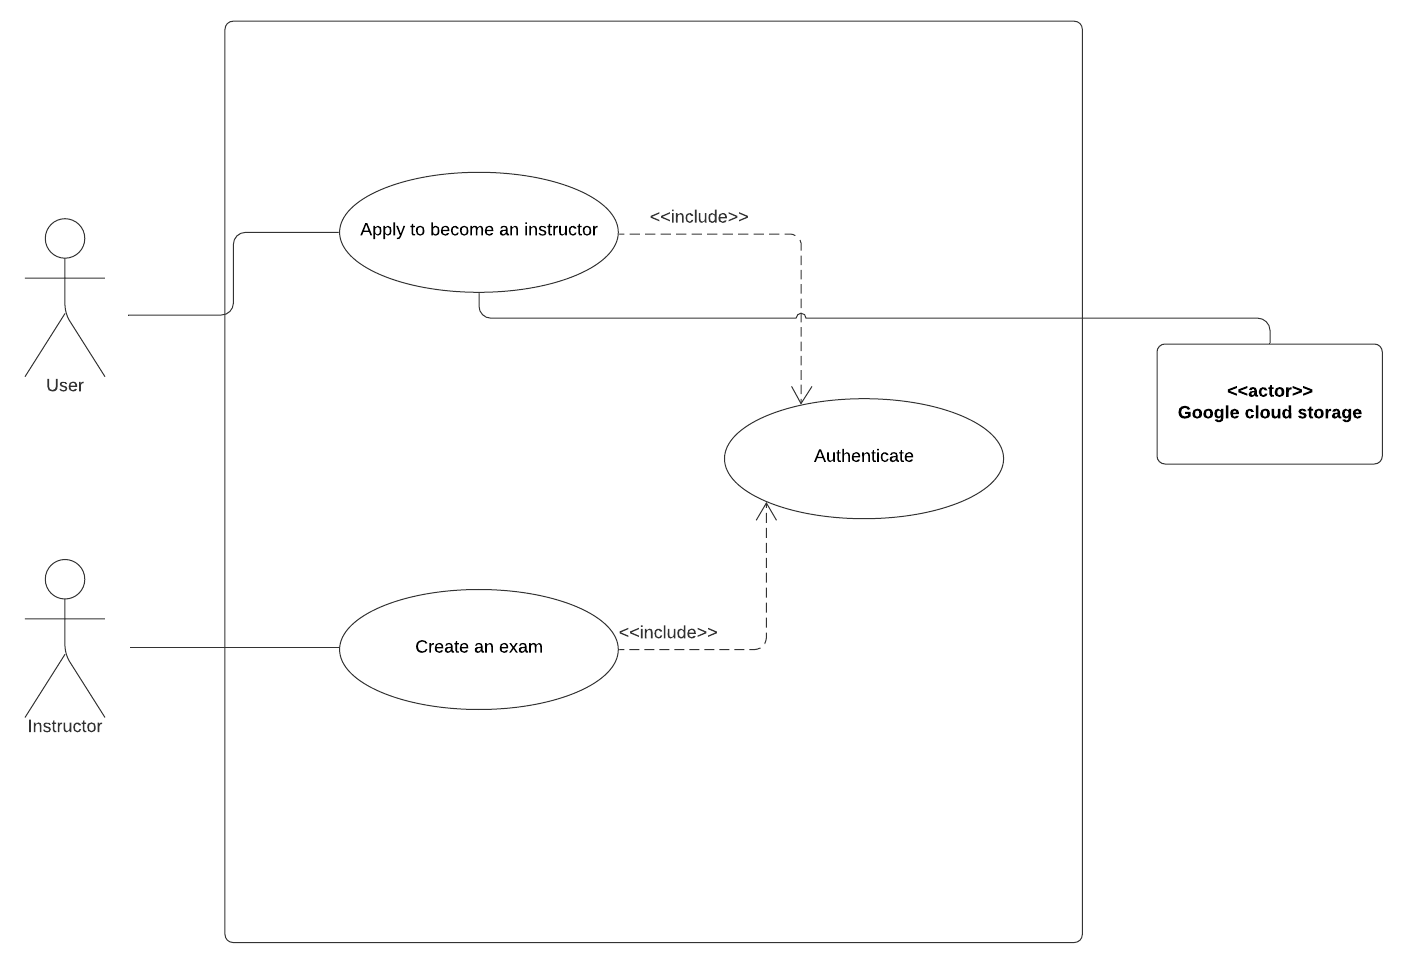
\includegraphics[width=130mm]{sprint3usecase.png}
    \caption{Sprint 3 use case diagram}
    \label{fig:sprint3usecase}
\end{figure}



\section{Modeling}

%%%%%table
\begin{table}[H]
\centering
\caption{create an exam textual description}
\begin{tabular}{|p{4cm}|p{10cm}|}
\hline
\textbf{\large{Use case name}} & Create an exam \\\hline
\textbf{\large{Actors}} & Instructor \\\hline
\textbf{\large{Preconditions}} & User logged in \\\hline
\textbf{\large{Postconditions}} & Exam created  \\\hline
\textbf{\large{Normal flow}} & 
\begin{itemize}
  \item The instructor visits the instructor space.
  \item The instructor clicks the course.
  \item The instructor clicks the exam link in the side bar.
  \item The instructor adds questions and answers.
\end{itemize}
\\\hline

\end{tabular}
\end{table}
%%%%%table

\begin{figure}[!ht]
    \centering
    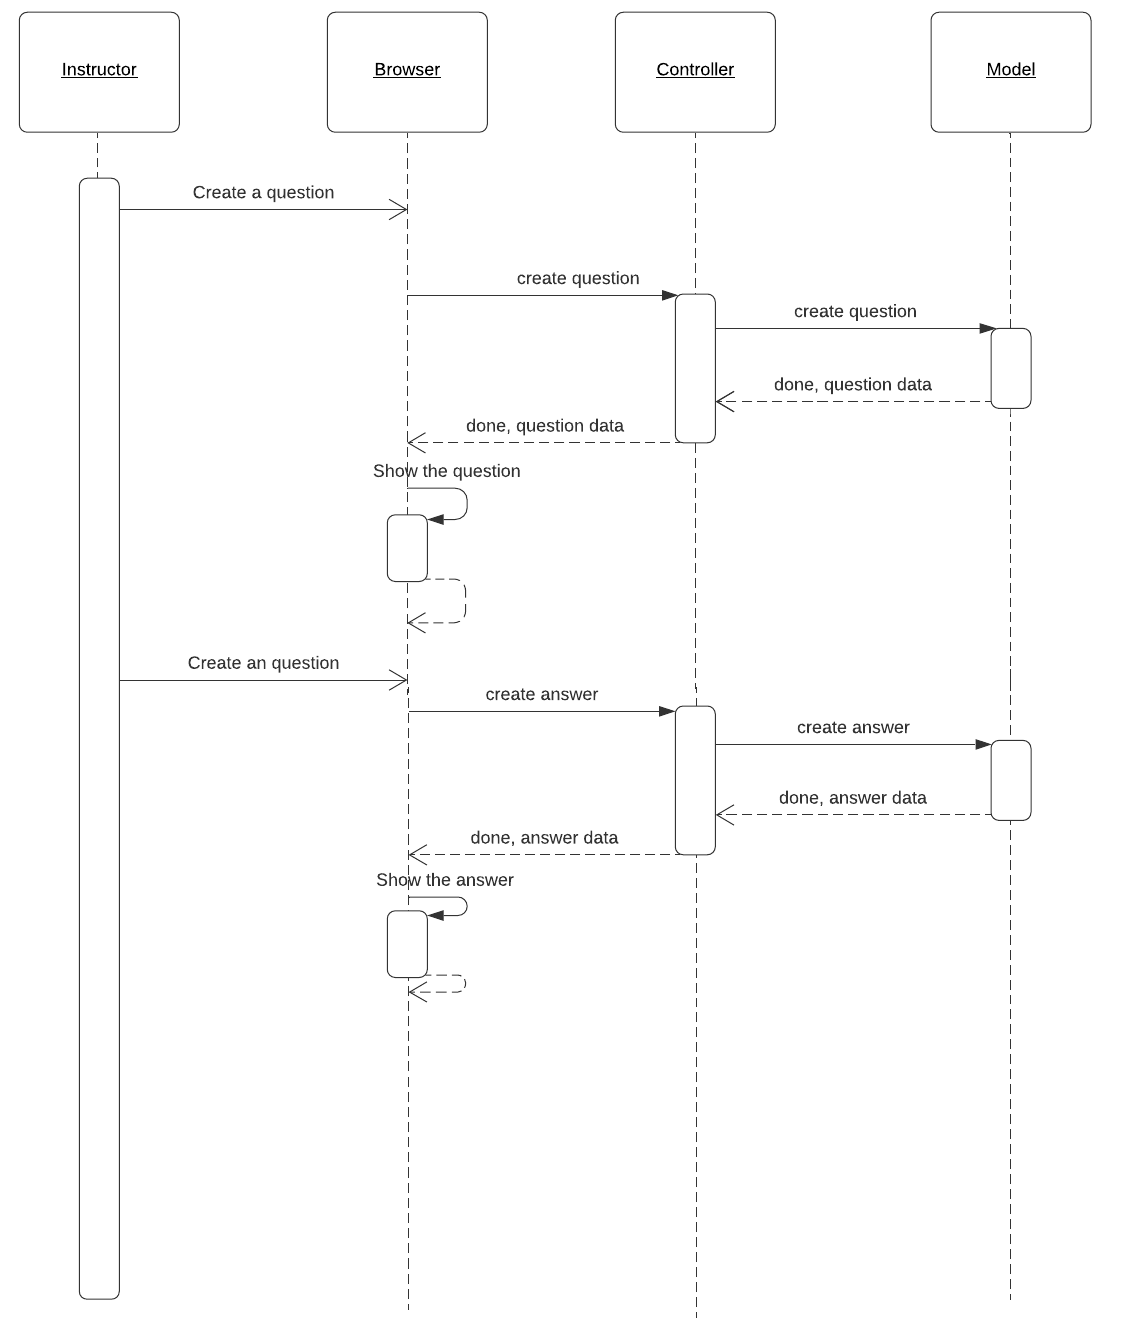
\includegraphics[width=142mm]{seq_create_exam.png}
    \caption{Sequence diagram of creating an exam}
    \label{fig:seq_create_exam}
\end{figure}


\vfill
\clearpage

%%%%%table
\begin{table}[H]
\centering
\caption{apply to become an instructor textual description}
\begin{tabular}{|p{4cm}|p{10cm}|}
\hline
\textbf{\large{Use case name}} & Recieve messages \\\hline
\textbf{\large{Actors}} & User \\\hline
\textbf{\large{Preconditions}} & User logged in \\\hline
\textbf{\large{Postconditions}} & Application sent \\\hline
\textbf{\large{Normal flow}} & 
\begin{itemize}
  \item The user visit the application form page.
  \item The user type the form data needed.
  \item The user submit the application.
\end{itemize}
\\\hline

\end{tabular}
\end{table}
%%%%%table

\begin{figure}[!ht]
    \centering
    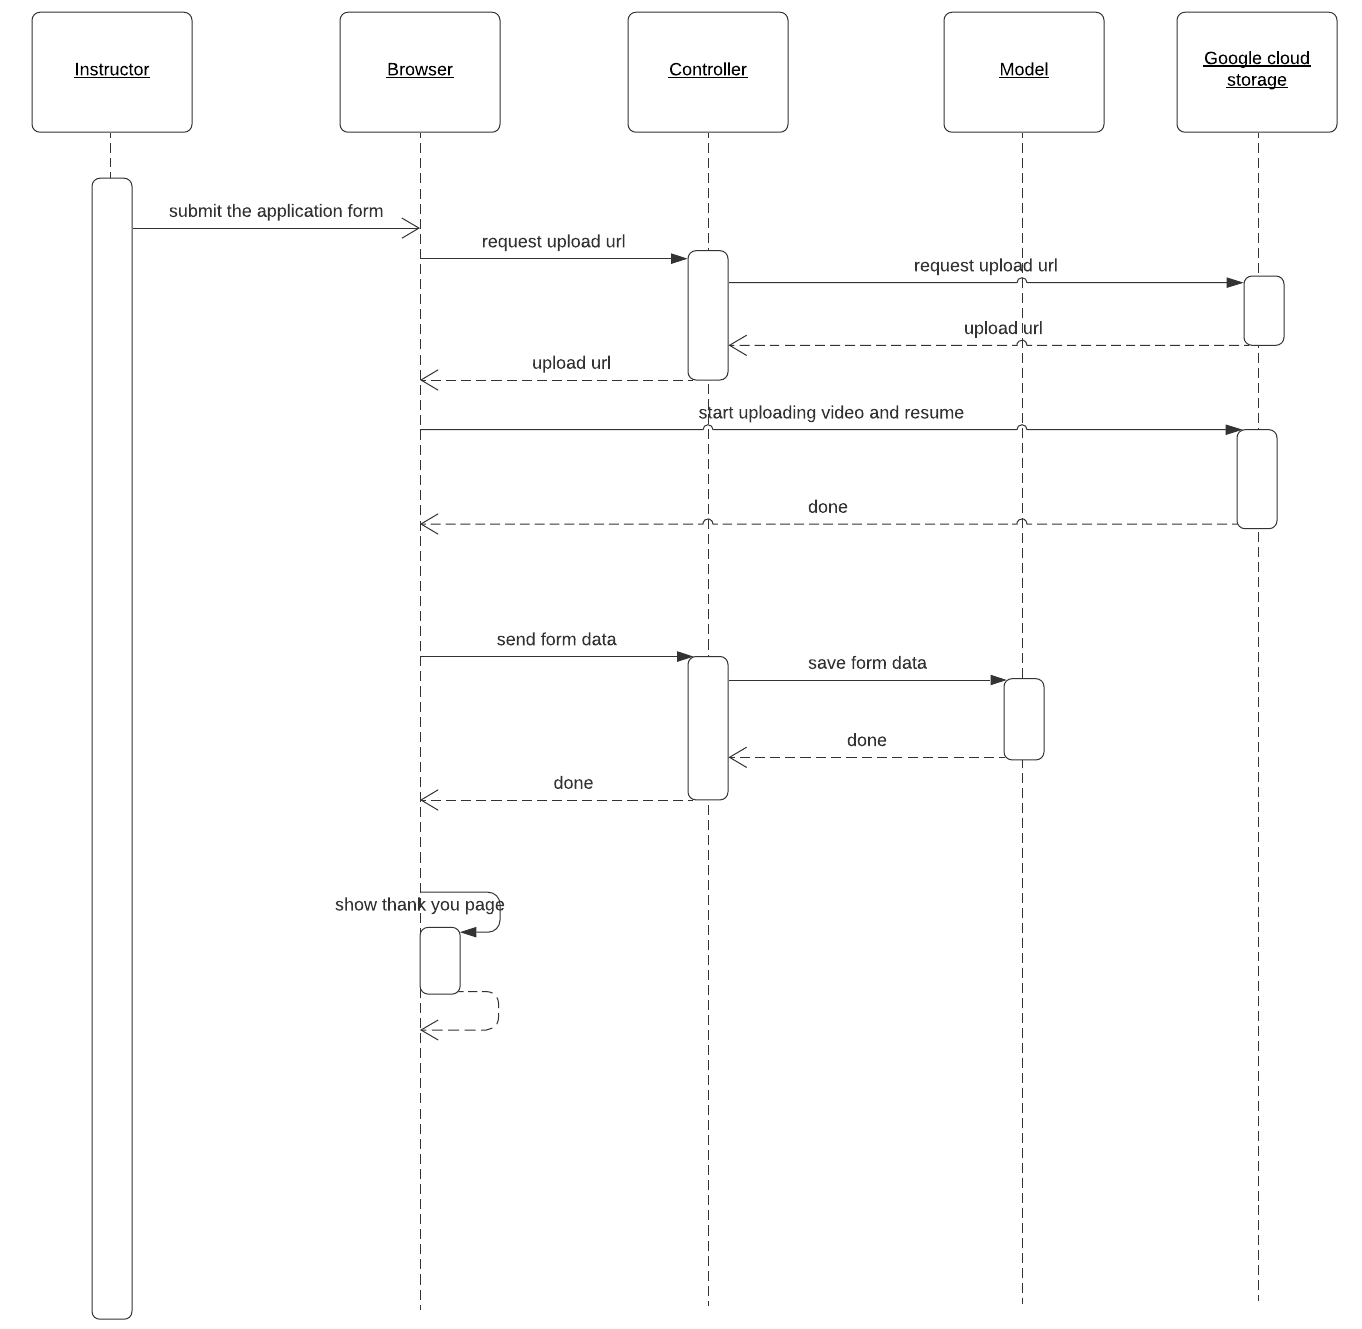
\includegraphics[width=150mm]{seq_apply_instructor.png}
    \caption{Sequence diagram of applying to become an instructor}
    \label{fig:seq_apply_instructor}
\end{figure}



\section{Implementation}
\subsection{Create an exam}
The instructor can manage and create an exam by clicking on the course and visiting the exam menu. An exam is composed of questions and questions have multiple answers and only one of them is correct.

To create a question, the instructor just needs type in the question and click add a question button which will fire a request to the server and in return we get the question data, we add that to the redux state to update the interface.

The user can also delete questions or answers which will make a request to delete the corresponding record and upon a successful request we remove the data the from redux state to update the interface.

\begin{figure}[!ht]
    \centering
    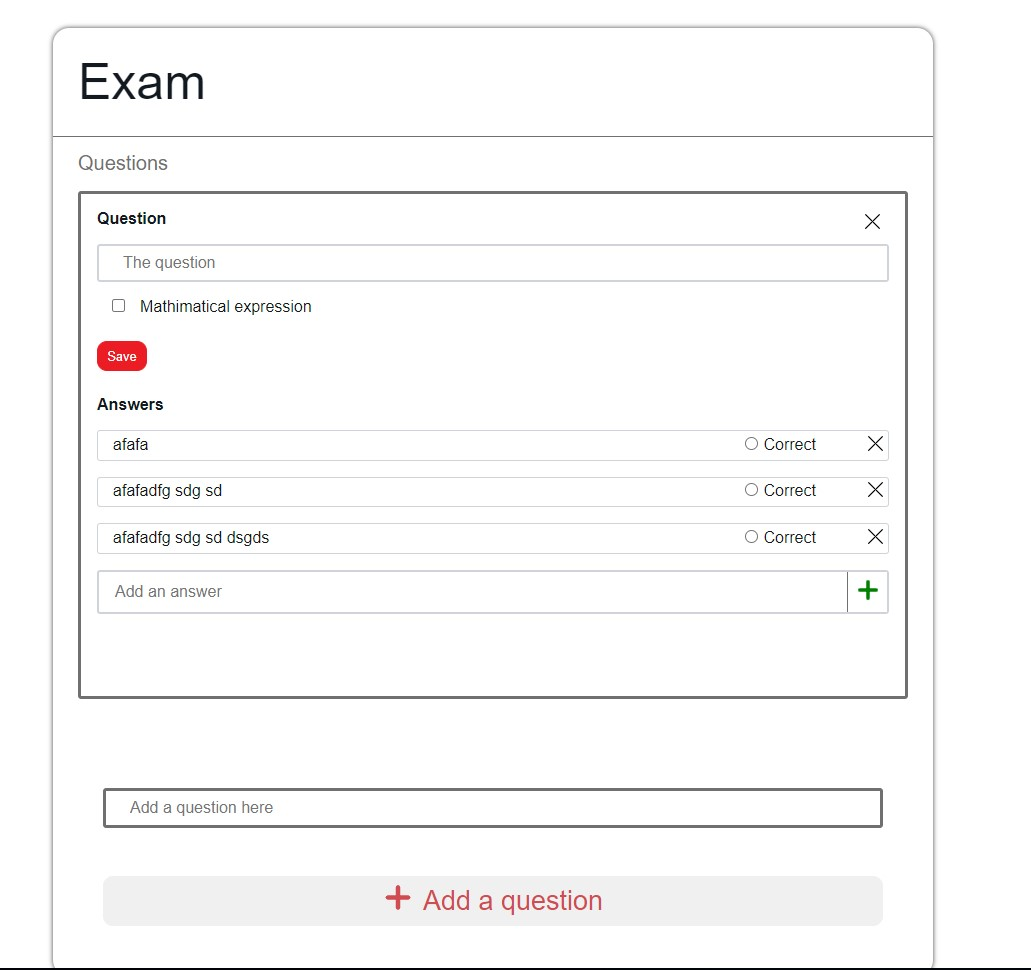
\includegraphics[width=150mm]{exam_form.jpg}
    \caption{Exam form interface}
    \label{fig:exam_form}
\end{figure}

\subsection{Apply to become an instructor}
If the current logged in user is not an instructor and tries to visit the instructor dashboard, he will be redirected to the instructor application form page.
When the user types the required form data and submits it, we request two upload url from the server and start uploading the cv and the video. Once it's done, we make a request to the server to save the submitted data.
\hfill \break
\hfill \break

\vfill
\clearpage

\begin{figure}[!ht]
    \centering
    
\includegraphics[width=150mm]{apply_instructor_1.jpg}
    \caption{Apply instructor page interface}
    \label{fig:apply_instructor_1}
\end{figure}


\hfill \break
\hfill \break
\hfill \break
\hfill \break

\begin{figure}[!ht]
    \centering
    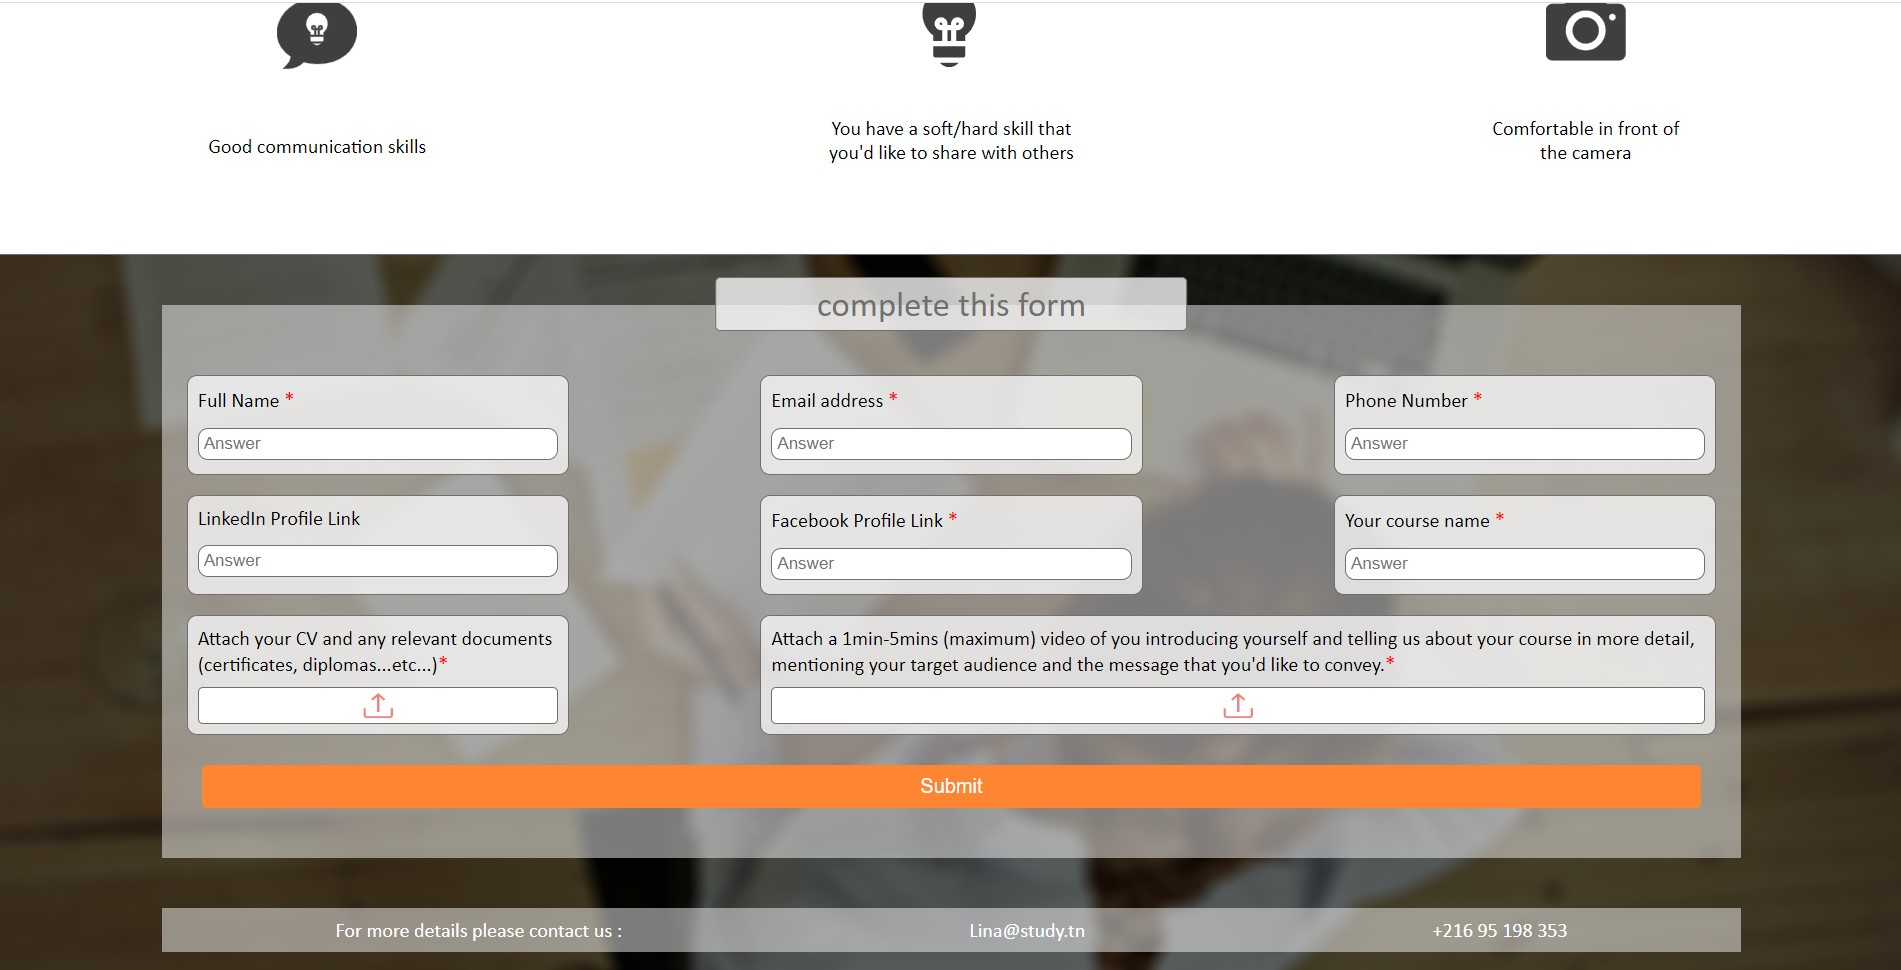
\includegraphics[width=150mm]{apply_instructor_2.jpg}
    \caption{Apply instructor form interface}
    \label{fig:apply_instructor_2}
\end{figure}


\vfill
\clearpage

\section*{Conclusion}
In this sprint, we have covered how the instructor can create an exam and how become an instructor.
\addcontentsline{toc}{section}{Conclusion}